\label{Principios de Machine Learning}
\section{Principios de Machine Learning}

Este trabajo integrador se incluyen campos de la inteligencia artificial, los cuales son Visión por Computadora y Deep Learning o Aprendizaje profundo. 
Esta sección tiene el propósito de hacer una introducción teórica a ambas ramas de la inteligencia artificial.

\subsection{Introducción: Visión por Computadora}
Una de las ramas de investigación más populares y utilizada de la Inteligencia Artificial es la Visión por Computadora o también llamada Computer Vision \cite{computervision1} \cite{computervision2} \cite{computervision3}.
Este campo se centra en intentar replicar funciones del sistema de visión humano, de forma que permita a las computadoras identificar y procesar objetos en imágenes o vídeos de forma similar a como los humanos lo hacen. Tiempo atrás, la capacidad de la visión por computadora era muy limitada, pero hoy en día hay muchas tecnologías que utilizan la visión por computadora, entre las cuales se encuentran el reconocimiento de objetos, la detección de sucesos, la reconstrucción de una escena y la restauración de imágenes.

En la actualidad, muchos son los campos que se han visto beneficiados por este conjunto de técnicas. Uno de los más conocidos es el de la robótica por medio de sensores o de cámaras, siendo estos últimos dispositivos idóneos para la aplicación de las estrategias de visión por computadora.

Sin embargo, podemos destacar otros ámbitos capaces de reconocer objetos, por ejemplo, en sistemas de seguridad, seguimiento de objetos o detección de anomalías en piezas fabricadas en una cadena de producción, medicina, etc.

\subsection{Fundamentos de Machine Learning}

Machine Learning \cite{ml}, es esencialmente un conjunto de algoritmos diseñado por un ser humano, pero que aprenden de los datos a los cuales son expuesto, dicho de otra manera, un conjunto de datos se usa para entrenar un modelo matemático de modo que cuando vea datos similares en el futuro, sepa reconocerlos. Los modelos, normalmente, toman datos como entrada y luego emiten una predicción de algo de interés. Estos algoritmos son ejecutados típicamente en algún tipo de computadora especial y sirven para resolver problemas de:
\begin{itemize}
    \item \textbf{Clasificación:} Retorna probabilidades de clase o distingue clases. Figura \ref{fig:clasificacion}.
    \item \textbf{Regresión:} Hace predicciones o estimaciones (en general numéricas). Figura \ref{fig:regresion}.
\end{itemize}

\begin{figure}[h!]
    \centering
    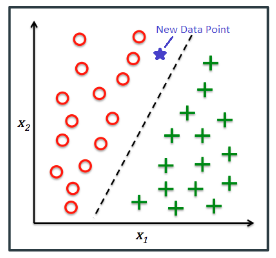
\includegraphics[width=0.5\textwidth]{img/clasificacion.png}
    \caption{Clasificación. Fuente: \cite{aprendisajesup}}
    \label{fig:clasificacion}
\end{figure}

\begin{figure}[h!]
    \centering
    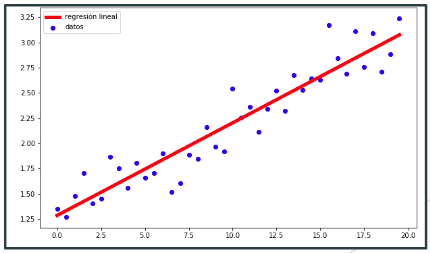
\includegraphics[width=0.8\textwidth]{img/regresion.png}
    \caption{Regresión. Fuente: \cite{aprendisajesup}}
    \label{fig:regresion}
\end{figure}

\newpage
El problema surge cuando se intenta resolver un problema de clasificación que no es linealmente separable. Aquí es donde aparecen la Redes Neuronales, con su capacidad de transformar estos problemas en linealmente separables. Figura \ref{fig:linealmente separables}.

\begin{figure}[h!]
    \centering
    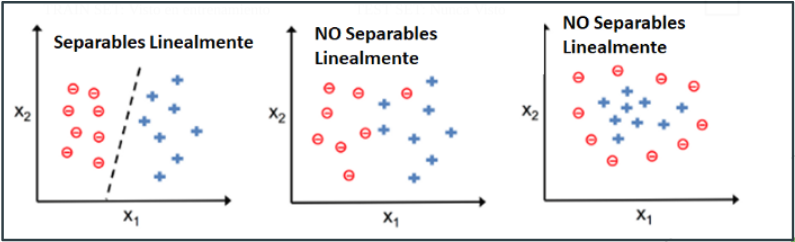
\includegraphics[width=1\textwidth]{img/linealmenteSeparable.png}
    \caption{Ejemplo Linealmente Separable. Fuente: \cite{aprendisajesup}}
    \label{fig:linealmente separables}
\end{figure}

\newpage
\paragraph{Ajuste del modelo: ¿Por qué se entrena un modelo de Machine Learning?}

Así como en la vida real a un ser humano se le enseña desde temprana edad a identificar distintos tipos de objetos dentro de su campo de visión, un modelo (o algoritmo) de Machine Learning tiene que aprender a detectar reconocer correctamente.

Para ello se lo entrena a partir de imágenes ya correctamente (ground truth) etiquetadas (bounding box) y, a grandes rasgos, si la predicción es correcta, se le alienta a seguir por ese camino y por el contrario si falla se lo alienta a ir en la dirección opuesta. Esto sería el ajuste con las perillas de una caja negra que viene a representar una abstracción de un modelo de Redes Neuronales, tal y como se representa en la siguiente Figura \ref{fig:abstraccion red neuronal}.

\begin{figure}[h]
    \centering
    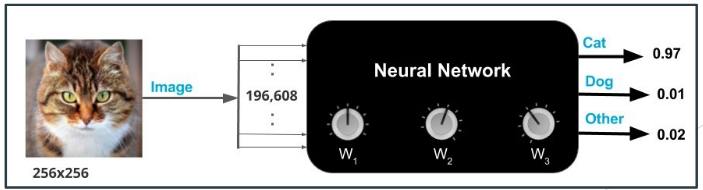
\includegraphics[width=1\textwidth]{img/RedNeuronal.png}
    \caption{Abstracción de una Red Neuronal. Fuente: \cite{redneuronalbasic}}
    \label{fig:abstraccion red neuronal}
\end{figure}

Se entrena el modelo a partir de un conjunto de datos lo suficientemente diverso, de tal manera que el modelo generalice y pueda realizar predicciones a partir de imágenes que nunca ``vio'' (analizó).

\begin{figure}[h!]
    \centering
    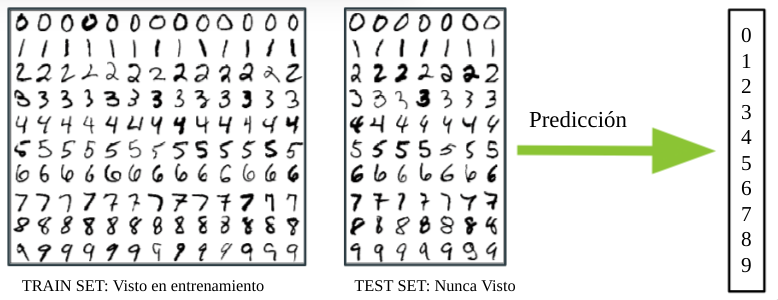
\includegraphics[width=1\textwidth]{img/RedNeuronal1.png}
    \caption{Ejemplo Machine Learning. Fuente: \cite{img_RedNeuronal1}}
    \label{fig:red neuronal 1}
\end{figure}

\subsection{Redes Neuronales}
Las Redes Neuronales Artificiales (ANNs por su siglas en inglés) son modelos matemáticos concebidos en un principio para estudiar (de cierta manera), el comportamiento del cerebro humano.
Estos modelos matemáticos son llamados Redes Neuronales porque fueron inspirados por neuronas biológicas, tal y como formalizaron: McCulloch y Pitts (1943) \cite{McCulloch1943-nf}; y Hebb & Hebb (1949) \cite{Morris1999-xd}. A grandes rasgos, se resume, que las Redes Neuronales Artificiales son formadas por circuitos neuronales y las interconexiones entre neuronas, llamadas sinapsis. Son llamadas sistemas conexionistas porque la información es codificada en los parámetros de las conexiones entre unidades.

En un principio, no hay una división clara entre conexionismo y neurociencia computacional, la principal diferencia es que los sistemas conexionistas se centran en procesos cognitivos de alto nivel, tales como: reconocimiento, memoria, comprensión  y razonamiento; en vez de detalles específicos del funcionamiento neuronal. En la década de 1980, el conexionismo experimentó una fuerte revitalización al formalizar una regla general de aprendizaje conocida como Backpropagation LeCun et al.(1988) \cite{lecun}. Backpropagation, que continua como el ``Hoyo en uno'' de la investigación conexionista contemporánea, permite a una amplia gama de modelos ANNs aprender una determinada función de mapeo de una entrada a una salida.

Hoy, el conexionismo esta mayormente englobado en el aprendizaje profundo (Deep Learning), ya que ha logrado  resultados notables en cuanto a avances en diversas aplicaciones. Aun no esta claro si las ANNs están limitadas en algún aspecto importante o no (por ejemplo, problemas de olvido catastrófico y ataques adversarios); sin embargo, está claro que los modelos de Deep Learning son lo suficientemente poderosos y flexibles para lidiar con muchos problemas.

En este capítulo, se introducen brevemente conceptos básicos relacionados al presente trabajo. Primero, se presentan las Redes Neuronales y su proceso de dos etapas (inferencia y entrenamiento). Luego, se introducen Clasificadores y otros modelos y técnicas esenciales para entender este trabajo. Finalmente, se presenta la literatura sobre Visión por Computadora y las métricas de evaluación centrales para medir la performance de los modelos de Machine Learning.

\subsection{Definición formal de Redes Neuronales}
En el aprendizaje supervisado, un dataset (conjunto de datos) de entrenamiento \mathbf{D = (xi, yi)}, representa a una función de mapeo (\mathbf{F : xi → yi}) definida por sus observaciones \textit{xi} y su correspondiente etiqueta \textit{yi}, que son variables independiente e idénticamente distribuidas (i.i.d) de una distribución \textit{Px},y. Luego, una red Neuronal es entrenada para aprender una función de mapeo \textit{f} que aproxima a \textit{F}. El objetivo de una Red Neuronal es relacionar correctamente las entradas \textit{xi} con las salidas \textit{yi}, mediante la adaptación de sus parámetros $\theta$. Por ejemplo, en un problema de clasificación de dígitos, \textit{xi} consiste en imágenes de dígitos mientras que \textit{yi} corresponde a la categoría del dígito.

% Definición: 
% Es un modelo matemático que consiste en un conjunto de unidades, llamadas neuronas artificiales, conectadas entre sí para transmitirse señales. 
% Formado por parámetros, entradas y una salida. 
% Una Red Neuronal podemos verla como una caja negra con una entrada, con una salida correcta, y cuenta con diferentes “perillas” que ajustan los parámetros que cambian las condiciones la red neuronal.

En dos pasos, un clasificador de redes Neuronales aprende una función de mapeo \mathbf{y = f(x; $\theta$)} y adapta los parámetros $\theta$ que minimiza las predicciones del modelo y la verdad absoluta.

El primer paso se llama propagación Feedfoward o inferencia. La información de entrada \textit{x} fluye a través de la red Neuronal, siendo multiplicada por sus computaciones intermedias hacia la salida. En la mayoría de los casos, el mapeo \mathbf{f(x) : x → y},  es una función de activación descripta por \mathbf{f(x) : g3 ◦ g2 ◦ g1(x)} donde \textit{gl} son las capas intermedias conectadas en cadena \mathbf{y = f(x) = g3(g2(g1(x)))}. Las capas intermedias son parametrizadas por un vector de pesos \textit{$\theta$l}, que es utilizado para ponderar la entrada antes de ser transformadas por la función de activación. En cada capa oculta, la función de activación transforma la suma ponderada de las entradas en una salida. Las capas ocultas pueden también contener parámetros \textit{bias} que son utilizados usualmente para desplazar la suma ponderada de la entrada. Una capa es comúnmente representada como: \mathbf{gl(x) = φ($\theta$l, x)} donde \textit{$\theta$l} es el parámetro de la capa y \textit{φ} es la función de activación de la capa. Una red neuronal comprende de una capa de entrada \textit{g1}, que es la primer capa de la red, una capa de salida \textit{g3} y varias capas intermedias. La ultima capa, la capa de salida, es donde se espera que esté la predicción.
El largo total de esta cadena representa la profundidad del modelo y es de donde proviene el termino aprendizaje profundo (Deep Learning).

Los datos de entrenamiento provistos, comprenden de observaciones de F evaluados a diferentes puntos. Cada muestra \textit{xi} es acompañada de una etiqueta \textit{yi = F(xi)}, que representa la salida deseada para la capa de salida. En conjunto, la etiqueta especifica qué debe ser la capa de salida. Sin embargo, el comportamiento de salida de las capas intermedias no esta directamente especificado por los datos de entrenamiento, por eso se llaman capaz ocultas.

El segundo paso, es llamado entrenamiento y consiste en ``enviar hacia atrás'' (backpropagation), una señal de error sobre los parámetros del modelo (Riedmiller and Braun (1993) \cite{Riedmiller1993ADA}). Una función de pérdida (Loss function), es utilizada para computar el error cometido por el modelo en sus predicciones; esto es, la pérdida es alta cuando el modelo esta haciendo un trabajo pobre y por el contrario es baja cuando está performando bien. La señal de error, es el valor de la diferencia entre las etiquetas predichas y las verdaderas etiquetas deseadas. Luego, este valor de error, es utilizado para ajustar los parámetros del modelo para reducir la discrepancia en la predicción. El gradiente de la función de perdida con respecto a capas previas, es utilizado como la regla de actualización para ajustar los parámetros de cada capa. El proceso de aprendizaje es repetido hasta converger, por lo que un optimizador iterativamente computa el gradiente sobre lotes aleatoriamente muestreados del set de entrenamiento. Cuando una red neuronal encuentra un set de parámetros ``óptimo'', está lista para ser desplegada y comenzar así, a hacer predicciones sobre ejemplos nunca antes observados.

Un amplio rango de características (features), permiten a las ANNs, enseñarle a \textit{f} a encontrar un mapeo válido entre las entradas y las salidas. Por ejemplo, para evadir limitaciones lineales, funciones no lineales $\Psi$ son utilizadas en capas ocultas en vez de transformaciones lineales, ya que provee mayores grados de libertad, que habilitan al modelo a ``entender'' las relaciones no lineales entre los ejemplos \textit{x} y sus correspondientes etiquetas \textit{y}. Las transformaciones no lineales, permiten transformar problemas no linealmente separables en linealmente separables. Más específicamente, las funciones no lineales, permiten al espacio de entrada ser doblado, por lo que éste espacio puede ser dividido en regiones lineales más pequeñas (Pascanu et al.(2013) \cite{pmlr-v28-pascanu13}). La transformación no lineal, la correcta función de perdida y un apropiado número de parámetros en las capas ocultas, permiten a la red neuronal, aproximar cualquier función de mapeo. Éste es el origen del término aproximado universal (Hornik et al. (1989)). Para una introducción detallada de Redes Neuronales, por favor referirse a Hornik et al. (1989) \cite{HORNIK1989359}.

La función de mapeo aprendida \textit{f($\theta$, x)}, es actualizada y evaluada todo el tiempo en aprendizaje continuo. Cuando se evalúa la performance de un clasificador, lo que es juzgado detrás de escena, es el grado de degradación de la función de mapeo relativa a la función original de mapeo F.

% \paragraph{Estructura de una Red Neuronal}\hfill \break

% Una red neuronal artificial es un grupo interconectado de nodos similar a la vasta red de neuronas en un cerebro biológico. 
% Consiste en un conjunto de unidades, llamadas neuronas artificiales, conectadas entre sí para transmitirse señales
% Cada nodo circular representa una neurona artificial y cada flecha representa una conexión ponderada (pesos -w-) desde la salida de una neurona a la entrada de otra. La información de entrada atraviesa la red neuronal (donde se somete a diversas operaciones) produciendo unos valores de salida.

% ================================================================
% \chapter{Capitulo 2}
% \label{Principios de Machine Learning}
% \setcounter{secnumdepth}{4}

% % \subsection{Feature extraction}

% % One of the most important abilities of the deep learning model comes from extensive feature engineering. Deep models disentangle as much of the input data as possible to find common patterns that allow them to establish similarities between seen and unseen samples.
% % Deep neural networks can be employed to extract these high-level representations of the input data. Among the neural networks employed to extract features, convolutional \ann{}s (CNNs) are a specialize kind of neural networks that allow extracting abstract representations of data \cite{lecun1989backpropagation}.
% % CNNs are neural networks that use convolutional and pooling operations in place of the general fully connected layers in at least one of their layers. The CNNs are often seen as feature maps because the output features of the CNNs are invariant to small local translations. The values (i.e. features) of most CNN layer outputs do not change for local input translations making CNNs very a attractive. For example, to determine whether an image contains a face, a CNN does not learn the location of the eyes with a pixel-perfect match. It only needs to learn that, if there is one eye on the left and one on the right, it is most likely a face. Interestingly, deeper feature maps encode high-level features like “trousers” or “humane eyes” while low-level feature maps detect edges and shapes from the raw input data.
% % Therefore, the deeper feature maps of a CNN contain common and invariant
% % patterns of the image class which are more informative than the raw input data; consequently, they facilitate many downstream tasks (e.g. object recognition and identification).

% % The feature extraction property of CNNs is not limited to CNNs, but is often a general property of deep models. For example, Transformers \cite{vaswani2017attention} neural networks are an attention-based mechanism with similar capabilities to CNNs in disentangling common patterns from input data. Moreover, it has recently been observed that fully connected neural networks can obtain competitive results in large-scale image classification tests, indicating their usefulness as feature extractors \cite{tolstikhin2021mlpmixer}. 
% % This work employs deep pre-trained deep models as an auxiliary tool to facilitate some experiments in Chapters 4 and 5.


% \section{Principios de Machine Learning}
    
%     \subsection{Como funciona. Introducción a Machine Learning}
%     Machine Learning:
%     \\
%     Es un conjunto de algoritmos que corren típicamente en algún tipo de computadora y sirven para resolver problemas de:
%         Clasificación: Retorna probabilidades de clase o distingue clases.
%         Regresión: Hace predicciones o estimaciones (en general numéricas)
    
%         \begin{figure}[h]
%         \caption{Clasificación}
%         \centering
%         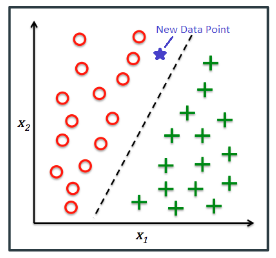
\includegraphics[width=0.4\textwidth]{img/clasificacion.png}
%         \end{figure}
    
%         \begin{figure}[h]
%         \caption{Regresión}
%         \centering
%         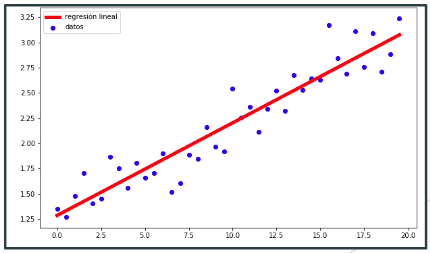
\includegraphics[width=0.6\textwidth]{img/regresion.png}
%         \end{figure}
        
%         El problema surge cuando se intenta resolver un problema de clasificación que no es linealmente separable.
%         Aquí es donde aparecen la Redes Neuronales, con su capacidad de transformar estos problemas en linealmente separables.
%         \begin{figure}[h]
%         \caption{Ejemplo Linealmente Separable}
%         \centering
%         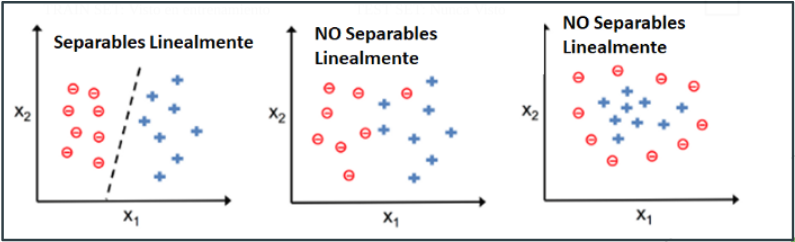
\includegraphics[width=0.9\textwidth]{img/linealmenteSeparable.png}
%         \end{figure}
        
%         \paragraph{Ajuste del modelo: ¿Por qué se entrena un modelo de Machine Learning?}\hfill \break
        
%         Así como en la vida real a un ser humano se le enseña desde temprana edad a identificar distintos tipos de objetos dentro de su campo de visión, un modelo (o algoritmo) de Machine Learning tiene que aprender a detectar objetos correctamente.
        
%         Para ello se lo entrena a partir de imágenes ya correctamente (ground truth) etiquetadas (bounding box) y, a grandes rasgos, si la predicción es correcta, se le alienta a seguir por ese camino y por el contrario si falla se lo alienta a ir en la dirección opuesta. Esto sería el ajuste con las perillas.
        
%         Se entrena el modelo a partir de un conjunto de datos lo suficientemente diverso, de tal manera que el modelo generalice y pueda realizar predicciones a partir de imágenes que nunca “vió”.
        
%         \begin{figure}[h]
%         \caption{Ejemplo Machine Learning}
%         \centering
%         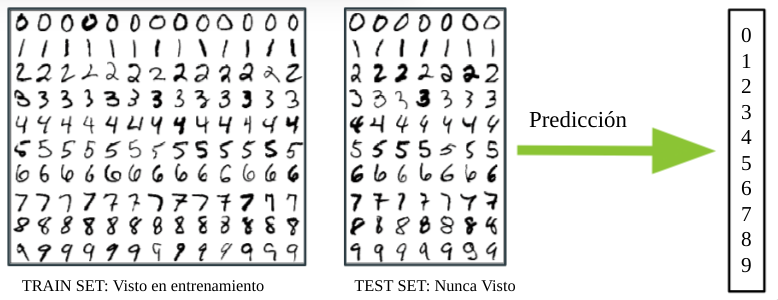
\includegraphics[width=0.9\textwidth]{img/RedNeuronal1.png}
%         \end{figure}
%     \subsection{Redes neuronales}
%         \subsubsection{Que es una red neuronal: Deep Learning}
%         \\
%         Definición: 
%         Es un modelo matemático que consiste en un conjunto de unidades, llamadas neuronas artificiales, conectadas entre sí para transmitirse señales. 
%         Formado por parámetros, entradas y una salida. 
%         Una Red Neuronal podemos verla como una caja negra con una entrada, con una salida correcta, y cuenta con diferentes “perillas” que ajustan los parámetros que cambian las condiciones la red neuronal.
        
%         \begin{figure}[h]
%         \caption{Ejemplo de una Red Neuronal}
%         \centering
%         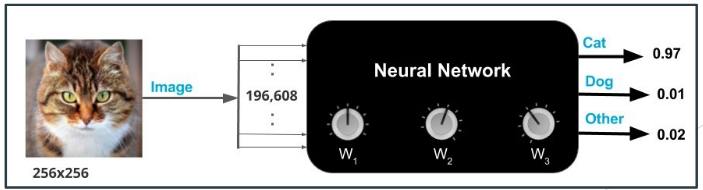
\includegraphics[width=0.9\textwidth]{img/RedNeuronal.png}
%         \end{figure}
        
       
%         \paragraph{Estructura de una Red Neuronal}\hfill \break
    
%         Una red neuronal artificial es un grupo interconectado de nodos similar a la vasta red de neuronas en un cerebro biológico. 
%         Consiste en un conjunto de unidades, llamadas neuronas artificiales, conectadas entre sí para transmitirse señales
%         Cada nodo circular representa una neurona artificial y cada flecha representa una conexión ponderada (pesos -w-) desde la salida de una neurona a la entrada de otra. La información de entrada atraviesa la red neuronal (donde se somete a diversas operaciones) produciendo unos valores de salida.
        
%         \begin{figure}[h]
%         \caption{Estructura de una Red Neuronal}
%         \centering
%         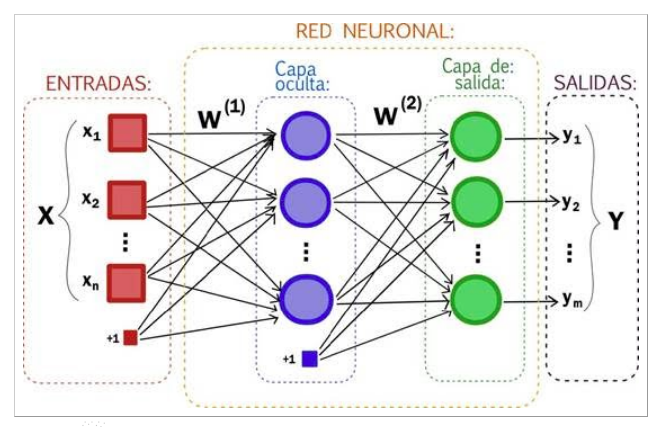
\includegraphics[width=0.8\textwidth]{img/RedNeuronal2.png}
%         \end{figure}
            
%             \paragraph{Que son la neuronas y como están conectadas}\hfill \break
            
%             \paragraph{¿Por que una Red Neuronal funciona?}
%                 \begin{enumerate}
%                 \item Función de activación\hfill \break
%                 En gran medida gracias a que tiene una Función de activación:
%                 Define la salida de un nodo dada una entrada o un conjunto de entradas. Por lo que decide si se activa la neurona o no.
%                 Matemáticamente se piensa como una multiplicación de matrices, es lo que en esencia transforma un problema no linealmente separable en uno linealmente separable.

%                 \begin{figure}[h]
%                 \caption{Función de Activación}
%                 \centering
%                 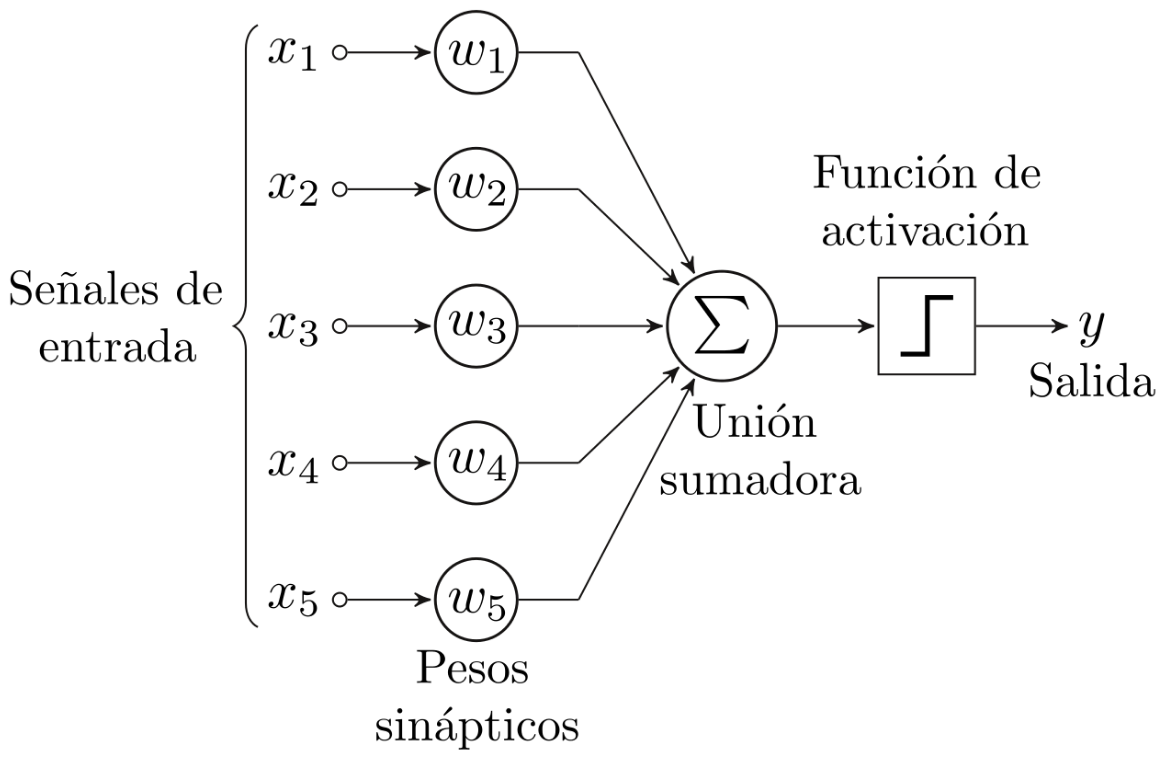
\includegraphics[width=0.8\textwidth]{img/FuncionActivacion.png}
%                 \end{figure}

%                 \item Que son las neuronas entonces\hfill \break
%                 Es una función que depende de los valores de las neuronas de la capa previa y retorna una salida, representado como un valor numérico real.
%                 Una Red Neuronal va a tomar un “estado de activación” el cual se ve reflejado en los valores que toman sus neuronas.
                
                
%                 \begin{figure}[h]
%                 \caption{Neuronas}
%                 \centering
%                 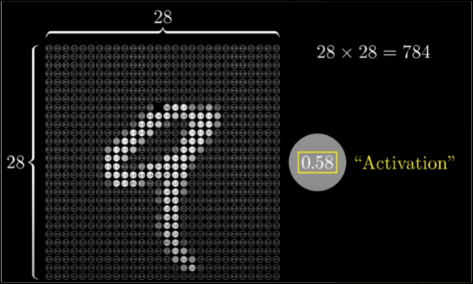
\includegraphics[width=0.8\textwidth]{img/neuronas.png}
%                 \end{figure}
%                 Ese número dentro de la neurona se llama "Activación" (o Activation en inglés). Para una imagen de 28x28 píxeles, los 784 píxeles ordenados como una lista de números conforman la primer "Capa" (o layer en inglés) de nuestra Red Neuronal. 

%                 La última capa de la Red Neuronal representa cada una de las distintas clases que queremos clasificar. En el ejemplo de detectar qué número es representado por una serie de números escritos a mano, tendríamos 10 clases, una por cada dígito del 0 al 9. 
%                 La activación de cada una de estas neuronas representa que tan seguro está el modelo de que la imágen a la entrada de la NN es un determinado dígito.
%                 También hay capas ocultas (hidden layers en inglés) entre la capa de entrada y la de salida que por el momento solo diremos que indican cómo este proceso de reconocer dígitos va a ser manejado.


        
%                 \end{enumerate}
%         \subsubsection{Gradient Descent, ¿cómo aprenden las Redes Neuronales?}
%             \paragraph{Introducción: La idea detrás del entrenamiento de una Red Neuronal}
%             \paragraph{¿Qué es entrenar una Red Neuronal? }\hfill \break
%             Es básicamente resolver un problema de optimización. Lo que se intenta es minimizar el error en la predicción (para ellos se utiliza el método de Gradient Descent).
%             Se intenta optimizar los pesos dentro de la red. La tarea es encontrar los pesos que mapean mejor la entrada de la red con su salida y éste mapeo es lo que la red debe aprender.

%                 \begin{enumerate}
%                 \item Función de costo\hfill \break
%                     La Función de Costo (o Loss Function en inglés) es un método de evaluación de que tan bien una Red Neuronal modela un determinado dataset. 
%                     Si la predicción se desvía mucho de los verdaderos valores, entonces la loss function toma un valor muy grande. 
%                     Gradualmente, con la ayuda de una función de optimización (como Gradient Descent), la loss function va ir reduciendo este error en la predicción a medida que la Red Neuronal va “aprendiendo”.\hfill \break

%                 \item Gradient Descent\hfill \break
%                     Gradient Descent: Su objetivo es minimizar la Función de Costo. Para obtener ese mínimo se calcula la derivada de la función de costo en un determinado punto y nos “movemos” en el sentido contrario al de la pendiente para acercarnos al mínimo local más cercano. Esto se hace ajustando los parámetros de la Red Neuronal. A medida que la pendiente se hace menos y menos pronunciada, los ajustes deben de ser más pequeños. 
                    
%                 \begin{figure}
%                 \caption{Gradiente Desccent}
%                 \centering
%               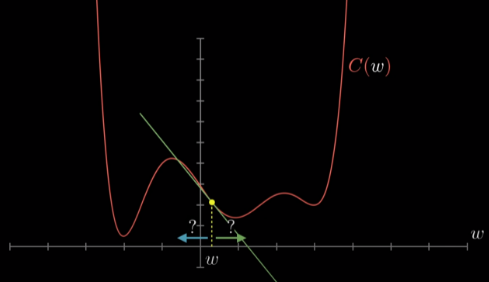
\includegraphics[width=0.7\textwidth]{img/GradienteDescent.png}
%                 \end{figure}\hfill \break
                    
%                     En la práctica, la función de costo depende de muchas variables (todos los pesos y bias de la NN) por lo que la pendiente en realidad se calcula como un gradiente en un punto dado de un plano multidimensional determinado por la función de costo.
                    
                   
%                 \begin{figure}[h]
%                 \caption{Gradiente Descent: Componentes}
%                 \centering
%                 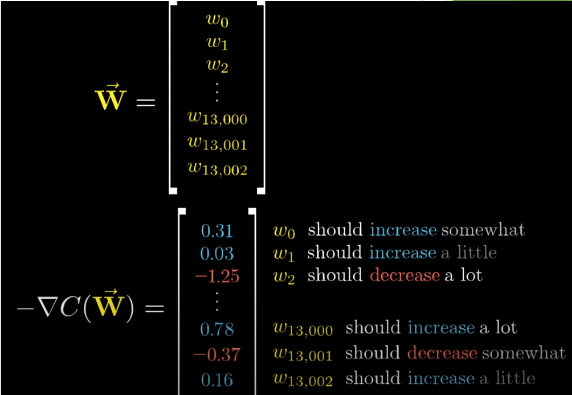
\includegraphics[width=0.7\textwidth]{img/GradienteDescent1.png}
%                 \end{figure}\hfill \break

%                 Cada componente del gradiente negativo nos indica 2 cosas:
%                 El signo nos indica si el peso asociado a dicho gradiente debe ser incrementado o disminuido.
%                 La magnitud del componente nos indica qué cambios en los pesos afectan más a la función de costo.
%                 \hfill \break
                
%                 \item Backpropagation - Stochastic Gradient Descent \hfill \break
                
%                 Es un algoritmo para computar el Gradient Descent y la clave de como una NN “aprende”. 
%                 Si recordamos, el valor que tiene una activación de la capa de salida depende de los pesos, el bias y las activaciones de la capa anterior. Esto es así para cada una de las activaciones, pero centrémonos un momento solo en una activación en particular. Si queremos que esa activación se parezca más al valor correcto de etiqueta, la clave está en modificar los parámetros que más afecten a esa activación de salida, en orden de disminuir el error y para lograrlo debemos alterar alguno de los 3 parámetros antes nombrados:
%                 \begin{itemize}
%                 \item Incrementando los bias
%                 \item Incrementando los pesos wi en proporción a la activación ai
%                 \item Cambiando las activaciones ai en proporción a los pesos wi que conectan con la capa previa
%                 \end{itemize}
%                 El problema está en que no podemos directamente inferir en los valores las activaciones individualmente, solo podemos controlar los pesos y bias.
%                 Pero este pensamiento nos sirve para saber qué necesita cada activación para poder clasificar correctamente.
%                 Por lo que se hace es una suma de lo que cada activación necesita ajustar; siempre teniendo en cuenta de ajustar proporcionalmente a lo que cada activación requiere para minimizar el error, y esa es la clave detrás del \textit{Backpropagation}.
                
%                 Ese vector promedio resulta ser el gradiente negativo de la Loss Function. En la práctica, para disminuir el costo computacional de calcular la influencia de cada uno de los ejemplos de entrenamiento en cada paso de gradient descent, por lo que se hace es:
%                 \begin{itemize}
%                 \item Mezclar aleatoriamente los ejemplos de entrenamiento.
%                 \item Dividirlos en mini-tandas (o “mini-batches”) de, digamos, 100 ejemplos.
%                 \item Ejecutar un paso de gradient descent (usando backpropagation) usando un mini-batch.
%                 \item Esto nos da un resultado aproximado de la mejor manera de acercarnos a ese mínimo local en la curva de la Cost function pero de una forma más computacionalmente efectiva.
%                 \end{itemize}
%                 A esto se lo llama Stochastic Gradient Descent.


%                 \end{enumerate}
                
% 	\subsection{Red neuronal convolucional (Convolutional neural network - CNN)}
% 		\subsubsection{Por que se usan}
% 		\subsubsection{Cimientos de las CNN}
% 	        \paragraph{Edge Detection}
% 		    \paragraph{Padding}
% 		    \paragraph{Strided Convolution}
% 		    \paragraph{Aclaración sobre la convolución en CNN}
% 		    \paragraph{Convolución multidimensional}
% 		    \paragraph{Tipos de Capas en CNN}
%                 \begin{enumerate}
%                     \item Convolucional (CONV)
%                     \item Pooling (POOL)
%                     \item Fully Connected (FC)
%                     \item SoftMax (SOFT)
%                 \end{enumerate}
% 	    \subsubsection{Deep Convolutional Models}
%     		\paragraph{Redes Neuronales Clásicas}
%     		    \begin{enumerate}
%         			\item LeNet-5
%         			\item AlexNet
%         			\item VGG-16
%     		    \end{enumerate}
%     		\paragraph{ResNet}
%     		\paragraph{Network in Network (1x1 convolution)}
%     		\paragraph{Inception Network}
% 	    \subsubsection{Consejos Prácticos al trabajar con CNN}
%     		\paragraph{Transfer Learning}
%     		\paragraph{Data Augmentation}
%     		\paragraph{Tips para mejorar la predicción}
%     		    \begin{enumerate}
%                     \item Ensembling
%                     \item Multicrop at test time
%                     \item Open Source
%                     \item Usar Modelos Pre-entrenado y tunearlos para nuestro dataset
%     		    \end{enumerate}
% 	        \paragraph{Transfer Learning}
% \newpage
